\section{Magnetized Target Fusion (MTF)}
\begin{frame} {Magnetized Target Fusion (MTF)}
    \begin{itemize}
        \item To obtain high pressure in magnetic confinement fusion (MCF): need to improve confinement time and/or enlarge the machine size.
        \item To obtain high pressure in inertial confinement fusion (ICF): compress small size plasma to ultra-high density but stability degrades the compression efficiency.
        \item MCF is a combination of MCF and ICF: compressing a magnetically confined plasma.
    \end{itemize}
\end{frame}

\begin{frame} {MTF Concept}
    \begin{figure}
        \centering
        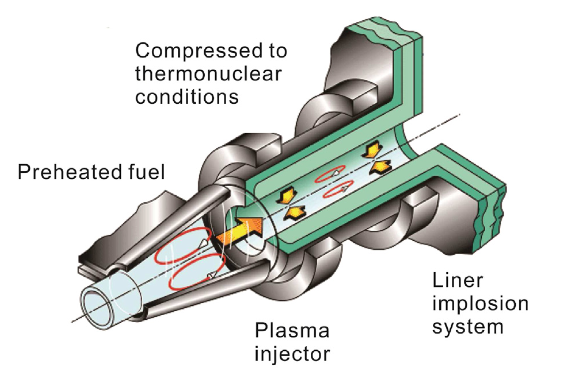
\includegraphics[width=0.6\textwidth]{figures/mtf-concept.png}
        \caption{Schematic of MTF concept. \cite{gao_2016_compact}}
        \label{fig:mtf-concept}
    \end{figure}

    \tiny \cite{gao_2016_compact} Z.Gao. \textit{Compact magnetic confinement fusion: Spherical torus and compact torus.}
\end{frame}

\begin{frame}[t] {MTF at General Fusion}
    \begin{wrapfigure}{l}{0.4\textwidth}
        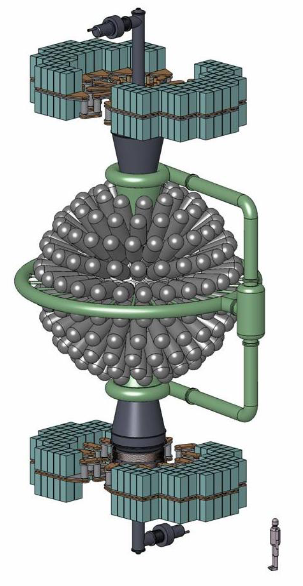
\includegraphics[height=0.6\textheight]{figures/mtf-at-general-fusion.png}
        \caption{General Fusion's Acoustic Magnetized Target Fusion Reactor Concept. \cite{delage_2012_progress}}
        \label{fig:mtf-at-general-fusion}
    \end{wrapfigure}

    The early MTF concept in General Fusion involves the compact torus.
    \begin{itemize}
        \item The deterium-tritium fuel is supplied as a pair of CTs (spheromaks).
        \item CT accelerators are at the poles.
        \item Injected CTs travel to the center and merge to form a stationary compressible plasma target.
        \item The target is compressed by acoustic pressure.
        \item The acoustic pulse is generated mechanically by hundreds of pneumatically-driven pistons.
    \end{itemize}

    \tiny \cite{delage_2012_progress}  M. Delage, A. Froese, D. Blondal, and D. Richardson. \textit{Progress towards acoustic magnetized target fusion: An overview of the r\&d program at general fusion.}
\end{frame}